%% IMPORTANT: Once working, run latex 3 times to get listoffigures to work

%% Be sure to check spelling!

%% Put **your** name and the proper due date in place

%% Copy the lstlisting and figure code as many times as you need
%% Be sure to put in your own file names if appropriate

%% Note that the \epsfig command is currently commented out - until the
%%%% files exist, processing this code without them will result in an error
%%%% so leave the comments until you have created the graphics files!

\documentclass{article}
\usepackage{amsmath}    % loads AMS-Math package
\usepackage{epsfig}     % allows PostScript files
\usepackage{listings}   % allows lstlisting environment
\usepackage{moreverb}   % allows listinginput environment
\usepackage[letterpaper, margin=0.75in]{geometry}  % set paper size/margins
\usepackage{textcomp}   % adds \interrobang, among others!

\begin{document}
\begin{center}
\rule{6.5in}{0.5mm}\\~\\
\textbf{\large EGR 103L -- Fall 2017}\\~\\
\textbf{\huge Structured Programming I}\\~\\
Ian Hanus (ih52)\\
Lab Section 1B, Tuesday 8:30-11:20 AM\\
1 October 2017\\~\\
{\small I understand and have adhered to all the tenets of the Duke
  Community Standard in completing every part of this assignment.  I
  understand that a violation of any part of the Standard on any part
  of this assignment can result in failure of this assignment, failure
  of this course, and/or suspension from Duke University.} 
\rule{6.5in}{0.5mm}\\
\end{center}
\tableofcontents
\listoffigures
\pagebreak

\section{Chapra Problem 2.10}
% Nothing to add here!
The code and the graph are in the appendices.

\section{Chapra Problem 2.22}
The equations for the butterfly curve\cite[p.~52]{Chapra} are:
\begin{align*}
x = \mbox{ sin}(t)(e^{\mathrm{cos}(t)}-2\mbox{cos}(4t)-\mbox{sin}^5(\frac{t}{12}))\\
y = \mbox{ cos}(t)(e^{\mathrm{cos}(t)}-2\mbox{cos}(4t)-\mbox{sin}^5(\frac{t}{12}))\\
\end{align*}
These equations generate a butterfly curve because of the sinusoidal nature of the sine and cosine graphs. The two long phrases in parentheses in the equation above match, so they simply determine the magnitude of the sin($t$) and cos($t$) graphs that distinguish x from y. The changing comparison of sin and cos at the different points make the butterfly appear.

\section{Palm Problem 3.12}
The equation for the length of the fence is:
\begin{align*}
\mbox{Length} =& \mathrm{Area}-\frac{1}{2}(\frac{\mathrm{Width}}{\sqrt{2}})^2\\
\end{align*}

Grading diary:
\listinginput[1]{1}{FenceDiary.txt}

\section{Pick a card!}
\listinginput[1]{1}{BTDiary.txt}

\section{What card is that?}
\listinginput[1]{1}{ITDiary.txt}

\section{Is that a three of a kind\textinterrobang}
\listinginput[1]{1}{TTDiary.txt}


\pagebreak
\appendix
\section{Codes}
% Put the name of your file in the subsection name 
% and the listinginput input
% Be sure to include the community standard in codes!
% Add \pagebreaks if they make sense

% Put the files in the same order as the problems; generally, 
% scripts will come first followed by any functions called
% by those scripts.
\subsection{RunChapra02p10.m}
\listinginput[1]{1}{RunChapra02p10.m}

\subsection{RunButterfly.m}
\listinginput[1]{1}{RunButterfly.m}

\subsection{Butterfly.m}
\listinginput[1]{1}{Butterfly.m}

\pagebreak

\subsection{FenceLength.m}
\listinginput[1]{1}{FenceLength.m}

\subsection{BuildCard.m}
\listinginput[1]{1}{BuildCard.m}

\pagebreak

\subsection{CardInfo.m}
\listinginput[1]{1}{CardInfo.m}

\pagebreak

\subsection{CheckTOK.m}
\listinginput[1]{1}{CheckTOK.m}
\clearpage % start Figures on new page

\section{Figures}
% Put the name of your file in the file= spot, 
% add a reasonable CAPTION, then be sure to 
% uncomment the epsfig line when the file exists 

% Put the figure in the same order as the problems

\begin{figure}[ht!]
\begin{center}
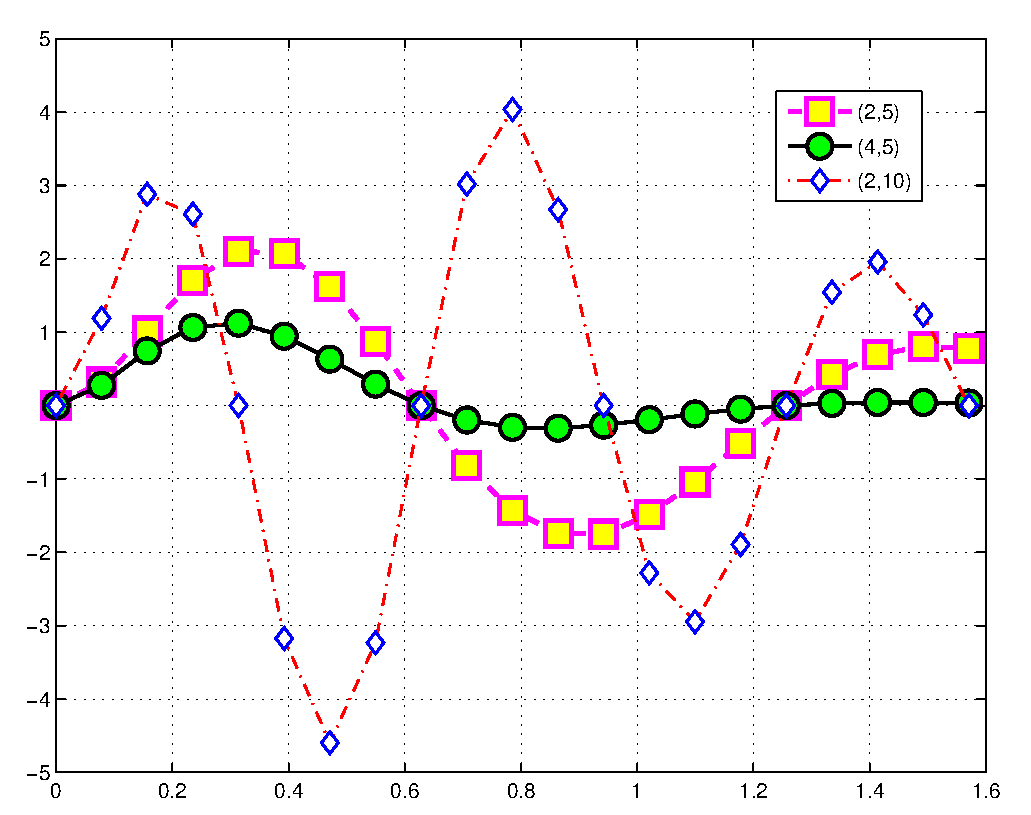
\epsfig{file=Chapra02p10Plot1.eps, width=4.5in}
\caption{Plot of Chapra Problem 2.10}
\end{center}
\end{figure}

\begin{figure}[ht!]
\begin{center}
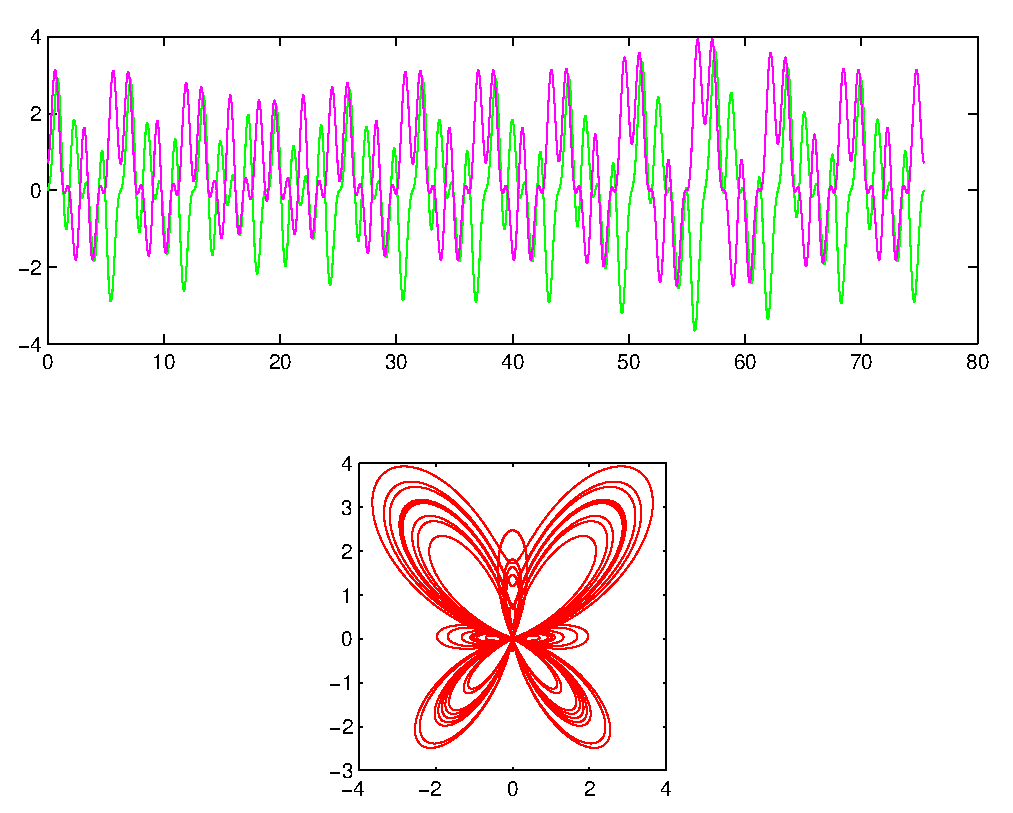
\epsfig{file=RunButterfly.eps, width=4.5in}
\caption{Plot of Butterfly Equations}
\end{center}
\end{figure}
\clearpage % start bibliography on new page

\begin{thebibliography}{9}
\bibitem{Chapra}
  Chapra, Steven C.,
  {\it Applied Numerical Methods with MATLAB for Engineering and Scientists}.
  McGraw-Hill, New York,
  4th Edition,
  2018.
\bibitem{Palm}
  Palm, William J.,
  {\it Introduction to MATLAB for Engineers}.
  McGraw-Hill, New York,
  3rd Edition,
  2011.
\end{thebibliography}

\end{document}
